% Planteamiento del Problema

\chapter{Marco referencial} % Chapter title

\label{ch:marcoReferencial} % For referencing the chapter elsewhere, use \autoref{ch:introduction} 
En este apartado se intenta recopillar la información para describir el \acrshort{CC} y los modelos de precios que usan los \acrshortpl{CCSP} para cobrar sus servicios.\bigskip

\section{Estado del arte}
Actualmente existen recursos de software para la orquestación de recursos en la nube, estos son bien conocidos como \acrfullpl{CROF}, han surgido como sistemas para gestionar el ciclo de vida de los recursos de multiples \acrshortpl{CCSP} y que cada vez exigen mecanismos de orquestación de recursos capaces de tratar con la heterogeneidad subyacente. \cite{tomarchio2020cloud}.\bigskip

\subsection{Tecnologías de orquestación}

\subsubsection{LibCloud}
Es una librería escrita en Python tiene licencia \emph{Apache 2.0}. Es una de las mas completas para administrar recursos de \acrshort{CC} teniendo unicamente carencias en el soporte de \acrshortpl{DBaaS} \footnote{\hyperref{https://medium.com/@anthonypjshaw/multi-cloud-what-are-the-options-part-1-low-level-abstraction-libraries-ce500f29120f}{}{}{https://medium.com/@anthonypjshaw}}. Esta librería oculta las diferencias entre las API de los \acrshortpl{CCSP} y permite administrar diferentes recursos de la nube a través de una \acrshort{API} unificada y facil de usar. \bigskip

Esta librería divide sus funciones en seis principales categorías\footnote{\url{https://libcloud.readthedocs.io/en/stable/index.html}}. La primera permite administrar Servidores en la nube y \emph{Block Storage}, este componente permite ejecutar secuencias de comandos para preparar al servidor recién creado. Otro tipo de recurso administrable es el almacenamiento de objetos en la nube \emph{Object Storage} y la administración de \acrshortpl{CDN}, Los servicios de balanceadores de carga \emph{Load Balancer}, la \acrshort{API} para administración de \acrshortpl{DNS} como servicio y los servicios de administración de Contenedores que permiten a los usuarios implementar y administrar contenedores usando software como \gls{Docker} con los proveedores que ofrecen una \acrshort{API} de \acrshort{CaaS}.\bigskip

\subsubsection{pkgCloud}
Es una librería escrita en \emph{Javascript} para usar sobre \emph{NodeJS}, al igual \emph{LibCloud} esta permite abstraer los diferentes mecanismos para acceder a las diferentes \acrshortpl{API} de los \acrshortpl{CCSP} para centralizar su administración, de manera adicional es la única librería con soporte de \acrshort{DBaaS}, permite integración con \emph{Rackspace} usando \emph{MySQL} y \gls{Microsoft Azure} con el servicio de \emph{Azure Tables}, esta librería tiene una licencia tipo \emph{MIT License} y además es un proyecto de colaboración disponible en \emph{GitHub}\footnote{\url{https://github.com/pkgcloud/pkgcloud}}.\bigskip

\subsubsection{Cloudify}
Es un \gls{Framework} que usa la arquitectura \emph{Multicloud} y el concepto de \acrfull{EaaS} usando \emph{Blueprints}. Los recursos y cargas de trabajo pueden ser orquestados y migrados en tiempo real entre diferentes \acrshortpl{CCSP}, su componente principal \emph{Cloudify Manager} permite administrar los recursos via interfaz web \emph{Cloudify Console}, este \gls{Framework} esta licenciado bajo \emph{Apache 2.0 License}, es uno de los \acrshortpl{CROF} mas completos gracias a su diseño lógico de \glspl{Plug-in} \footnote{\url{https://github.com/orgs/cloudify-cosmo/repositories}}.\bigskip

\subsubsection{Terraform}
Es una herramienta de \acrfullpl{IaaC} que aprovisiona y administra infraestructuras usando un lenguaje de configuración de alto nivel, \emph{Terraform} puede administrar múltiples proveedores de nube e incluso dependencias entre \acrshortpl{CCSP}, \emph{Terraform} aprovecha los \acrshortpl{CCSP} para proporcionar capacidades de escalado automático con disparadores de umbral en las métricas del sistema recopiladas por los servicios de monitoreo \cite[p.14]{tomarchio2020cloud}. \bigskip


\subsection{Costos de servicio}
\subsubsection{\acrlong{AWS}}
Este \acrshort{CCSP} tiene una página web en la \autoref{fig:AWS} dedicada para el cálculo de los costos de sus servicios \footnote{\url{https://calculator.aws}}, la página permite la estimación de los recursos seleccionando uno o varios servicios y estableciendo su configuración para después exportarla en un \acrfull{PDF}
\begin{figure}[h]
    \centering
    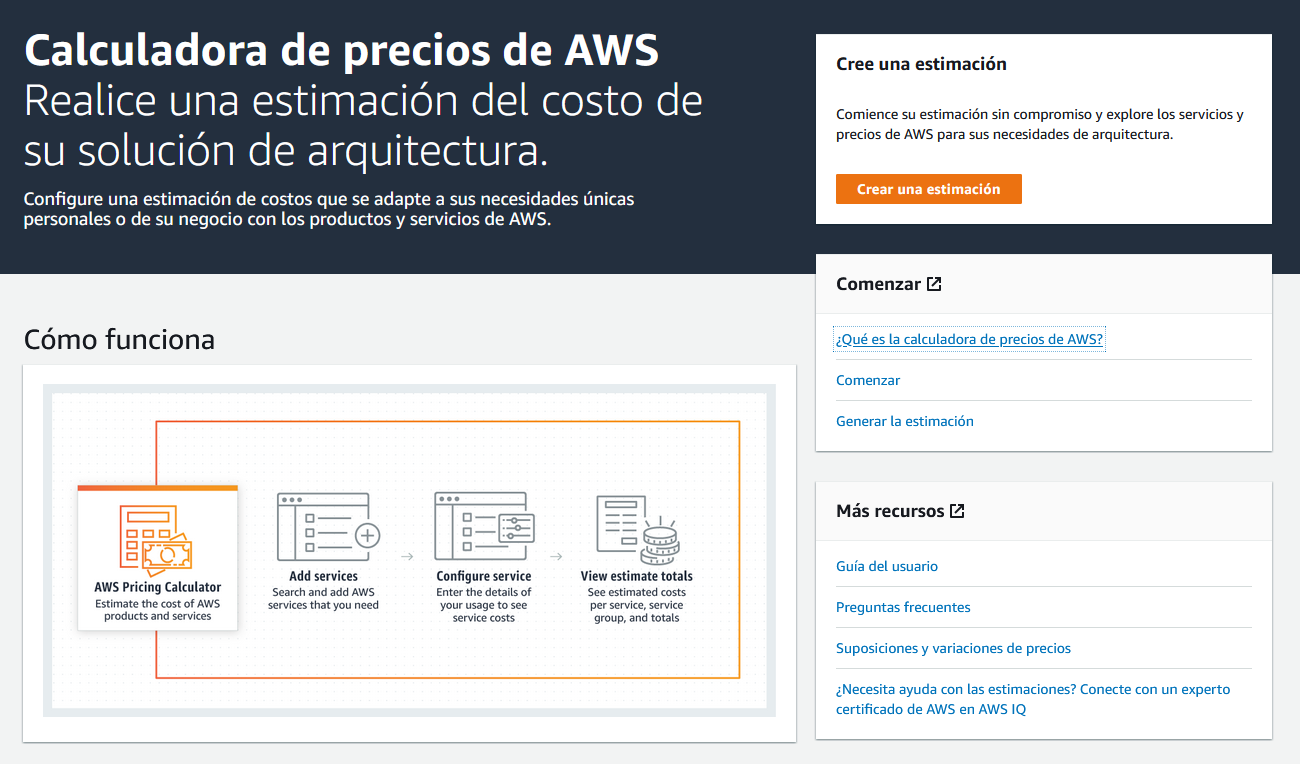
\includegraphics[width=\textwidth]{gfx/calculatorAws.png}
    \caption{Pagina de precios de \acrshort{AWS}}
    \label{fig:AWS}
\end{figure}

\subsubsection{Google Cloud}
También conocido como \acrfull{GCP} este \acrshort{CCSP} tiene un sitio web\footnote{\url{https://cloud.google.com/pricing}} con una calculadora de estimación en la \autoref{fig:GCP}, también es posible acceder los precios usando una lista de precios dinámica para cada tipo de servicio mostrando su costo de operación por hora e incluso con algunas ofertas gratuitas para la capa mínima de servicios\footnote{\url{https://cloud.google.com/pricing/list}}.
\begin{figure}[h]
    \centering
    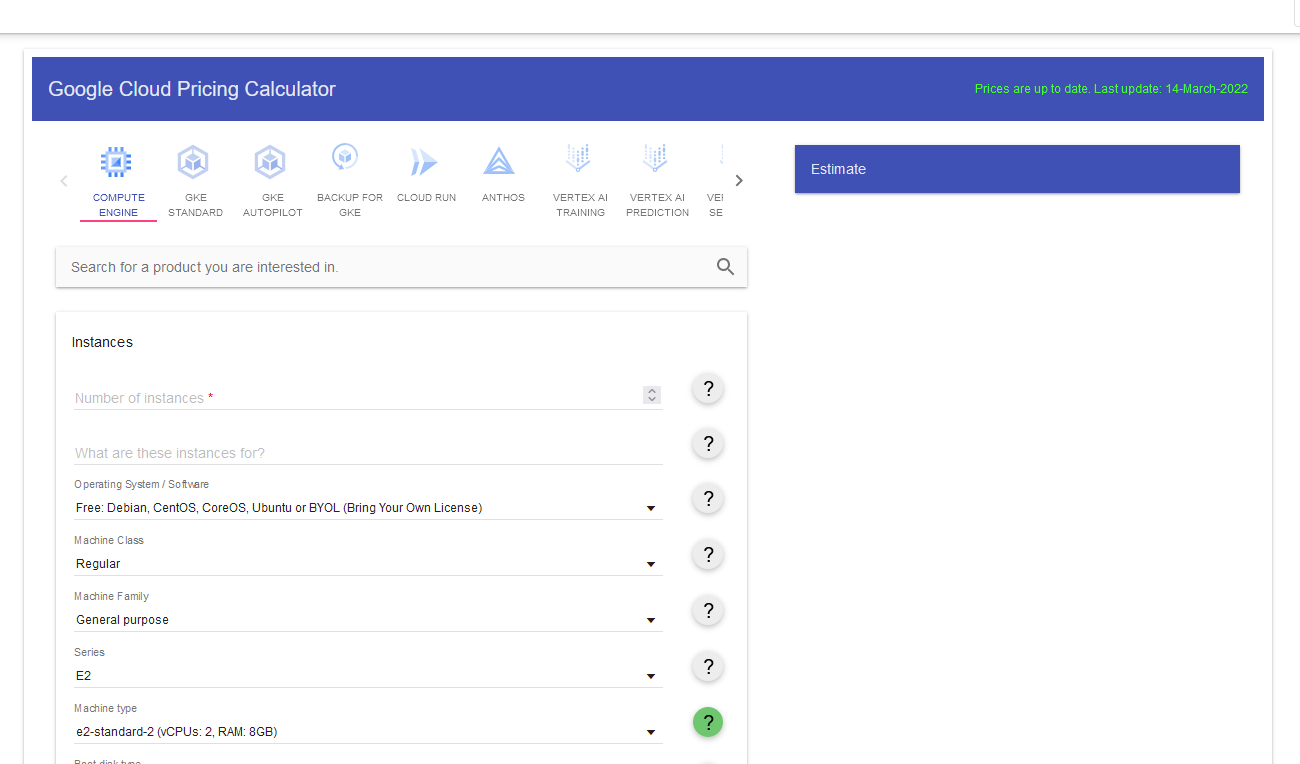
\includegraphics[width=\textwidth]{gfx/calculatorGCP.png}
    \caption{Pagina de precios de \acrshort{GCP}}
    \label{fig:GCP}
\end{figure}

\subsubsection{Microsoft Azure}
Al igual que los demas \acrshort{CCSP} \gls{Microsoft Azure} tiene una calculadora y lista dinámica de precios \footnote{\url{https://azure.microsoft.com/es-es/pricing/}} que puede ser consultada en términos de los servicios con el modelos de cobro por horas con se ve en la \autoref{fig:azure}.
\begin{figure}[h]
    \centering
    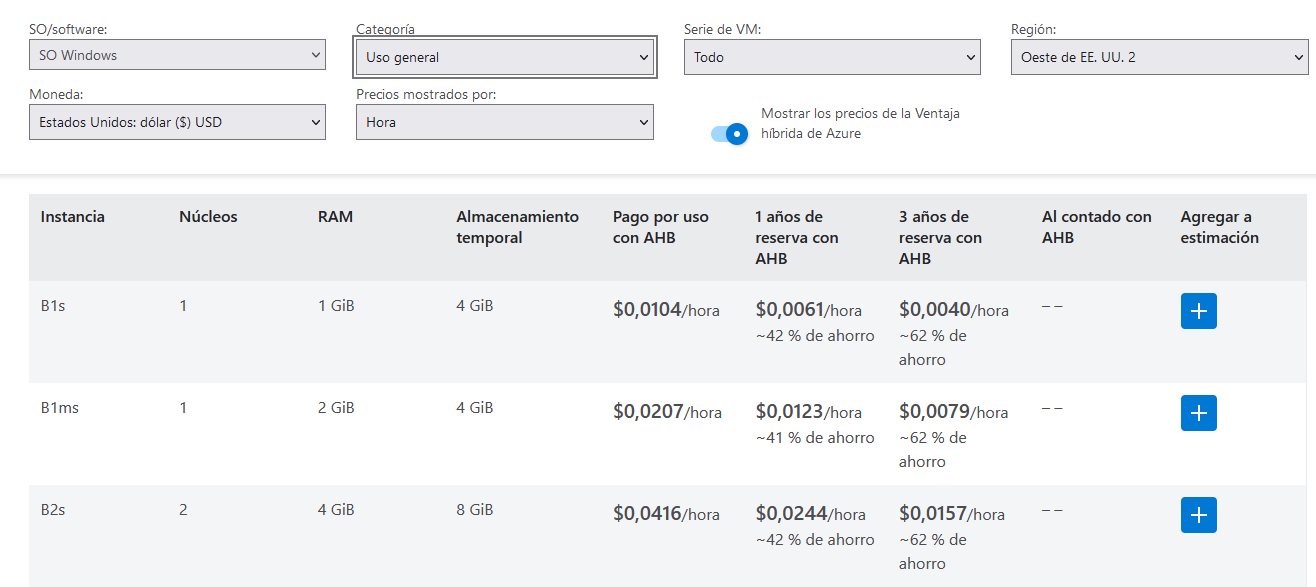
\includegraphics[width=\textwidth]{gfx/azure.png}
    \caption{Lista de precios de \gls{Microsoft Azure} para \acrshortpl{VM} con \acrshort{OS} \emph{Windows}}
    \label{fig:azure}
\end{figure}

\subsubsection{Oracle Cloud Infrastructure}
Orace tiene un estimador de costos y lista de precios en su sitio web.\footnote {\url{https://www.oracle.com/co/cloud/price-list.html}} como se muestra en la \autoref{fig:oracle}.
\begin{figure}[h]
    \centering
    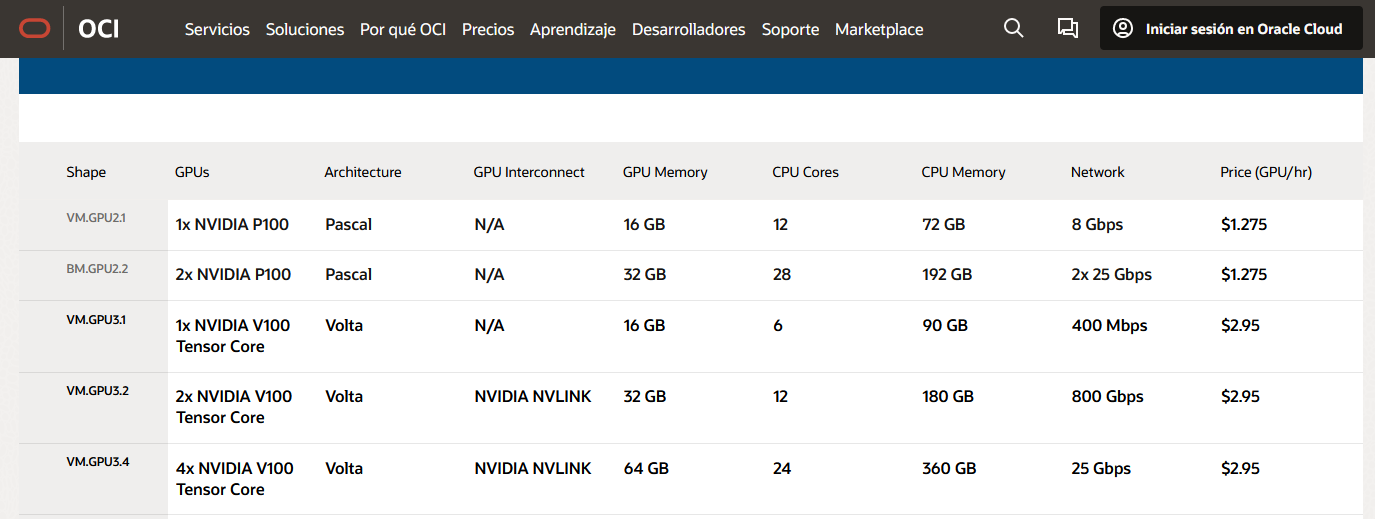
\includegraphics[width=\textwidth]{gfx/oracle.png}
    \caption{Muestra de precios para instancias de \acrshort{GPU} de \emph{Oracle Cloud}}
    \label{fig:oracle}
\end{figure}

\section{Marco teórico}
\subsection{Cloud Computing}
Según el \acrshort{NIST} la computación en la nube está definida como un modelo que permite el acceso de red conveniente y bajo demanda a un grupo compartido de recursos informáticos configurables como redes, servidores, almacenamiento, aplicaciones y servicios que pueden aprovisionarse y librerarse rápidamente con un mínimo esfuerzo de gestión o interacción con el \acrshort{CCSP}\cite{liu2011nist}.
\bigskip

%Hablar de los tipos de nubes
\subsubsection{Modelos de despliegue}
En el \acrshort{CC} existen varios modelos de despligue dependiendo de cual es el alcance de los recursos. La \emph{Nube privada} donde los datos y procesos son administrados dentro de la organización quien también se encarga de dar mantenimiento a la infraestructura que recide en las mismas instalaciones o en un lugar remoto administardo por la organización. En la \emph{Nube pública} los recursos son aprovisionados dinamicamente a través de Internet, el \acrshort{CCSP} le permite acceder a los todos los tipos de servicios bajo esquemas de pago por uso. En una \emph{Nube híbrida} los recursos o servicios de la organización pueden ser complementarios entre ambas ubicaciones e incluso pueden incluir infraestructura de \emph{Edge Computing} como dispositivos de \acrshort{IoT} \cite[p.2]{choudhary2007software}.

\subsubsection{Tipos de servicios}
Los servicios servicios de \acrshort{CC} ofrecen mas beneficios que la computación tradicional, ahorro de costos, escalabilidad, almacenamiento movil, acceso desde cualquier momento o cualquier lugar, mejor seguridad, ahorro de energía\cite{sether2016cloud}. En terminos de taxonomía el \acrshort{CC} está divido en tres principales tipos de servicios, \acrfull{IaaS} que puede verse como una evolución de los \acrfullpl{VPS} la cual ofrece plataformas de virtualización donde los clientes deben configurar sus propio software, estos servicios son facturados con base en los recursos consumidos, el modelo de pago por alquiler permite usar hasta mínimo una hora en algunos casos donde la cantidad de instancias se duplican para satisfacer las necesidades los clientes. Entre los tipos de soluciones que se encuentran en esta categoría están \acrfull{EC2}, \emph{Rackspace Cloud}, \emph{IBM Smart Bussiness Cloud solutions}, \emph{Oracle Cloud Computing}, \emph{Google Compute Engine}. \cite[p.2]{sether2016cloud}\bigskip

Otro esquema de servicios ofrecidos por el \acrshort{CC} son las  \acrfullpl{PaaS}, como características principales tenemos que son proveidas a los clientes por una interfaz en un navegador para editar, depurar, desplegar y monitorear una aplicación.\cite[p.1]{lawton2008developing} A diferencia de las \acrshortpl{IaaS} permiten una interacción de alto nivel con el cliente porque abstraen la configuración del entorno donde se ejecutan las aplicaciones, ademas de permitir la preconfiguración de un entorno de ejecución para un lenguaje de programación específico. Entre los \acrshortpl{CCSP} mas conocidos se encuentra también \acrshort{EC2} con la posibilidad de preconfigurar los entornos,  \emph{Salesforce.com} y \emph{Google App Engine}. \bigskip

El siguiente nivel en terminos de abstracción son las \acrfullpl{FaaS} conocidas también como computación \emph{Serverless} \cite[p.1]{lynn2017preliminary} que emerge como un paradigma conveniente para el despliegue de aplicaciones y servicios donde el desarrollador no se preocupa acerca de los aspectos operacionales, de despliegue, y mantenimiento y espera de este que sea tolerante a fallos y auto escalable especialmente el código que es escalable a cero donde no hay servidores corriendo cuando la función del usuario no está siendo usada. \acrshort{FaaS} a diferencia de \acrfullpl{PaaS} evita que el cliente reciba cobros en los periodos de inactividad de la función.\cite[p.5]{Baldini2017} Entre los servicios mas conocidos están \emph{Azure Functions}, \acrshort{AWS} \emph{Lambda}, \emph{Google Cloud Functions} y \emph{Oracle Cloud Functions}.\bigskip

Por último y mas cerca del usuario se encuentran el \acrfull{SaaS}, en este modelo de servicios el cliente interactúa con una aplicación que da soporte a los procesos de su modelo de negocío o le ofrece un servicio, el cliente paga recurrentemente por las funcionalidades y la cantidad de usuarios que usan el servicio, el \acrshort{SaaS} presenta ventajas frente al software tradicional, el cliente compra una suscripción y no una licencia perpetua, además el software tradicional tarda algunos años en publicar una nueva versión que el \acrshort{SaaS} puede poner a disposición en cuanto esté completa \cite[p.1]{choudhary2007software}. Algunos ejemplos de \acrshortpl{SaaS} son \emph{Google Workspace}, \emph{Microsoft 365}. \bigskip

\subsection{Modelos de precios}
De manera general existen dos grupos de modelos de precios, los modelos de \emph{precios dinámicos} donde el costo es flexible y depende de factores como el número de peticiones, el espacio usado, el tráfico generado, el poder de cómputo requerido o la cantidad de instancias necesarias. En los modelos de \emph{precios fijos} se dice que el cliente tiene mayor seguridad sobre el costo del servicios porque tiene un cargo fijo periodicamente para pagar, sin embargo el beneficio nunca es real porque depende del uso que tenga el servicio contratado donde algunas veces puede llegar al sobreuso.\cite[p.4]{soni2017pricing}.\bigskip


Los \acrshortpl{CCSP} usan modelos de precios mixtos que incluyen el esquema de pago por suscripción y el pago por uso, \emph{Pay-as-you-go} que usan las \acrshortpl{IaaS} y las \acrshortpl{PaaS}. \bigskip

Existen otros modelos como el \emph{Modelo de pago por suscripción} donde los precios se establecen de acuerdo con el nivel de la suscripción, son comunmente usados por los provedores de servicios de \gls{Hosting}. El \emph{modelo de pago basado en costos} permite al \acrshort{CCSP} calcular los precios dinámicos dependiendo de la demanda y las operaciones del los centros de datos del \acrshort{CCSP}. Entre los demás modelos de precios dinámicos están los \emph{Modelos genéticos de precios}, \emph{Modelos de precios basados en la competencia}, \emph{Modelos de precios basados en el cliente}, \emph{Modelos de precios con subasta dinámica} y los \emph{Modelos de precios híbridos} que establecen el precio con la convinación de los mencionados anteriormente\cite[p.7]{soni2017pricing}.


